%\documentclass[pldi]{sigplanconf-pldi16}
%\documentclass[10pt]{usenix}
\documentclass[10pt]{sigplanconf}
%\usepackage{usenix,epsfig,endnotes}

%\usepackage{epsfig,endnotes}
% standard LaTeX packages
%\usepackage{changebar}
\usepackage[normalem]{ulem}
\usepackage{algorithm}
\usepackage{algpseudocode}
\usepackage{balance}
\usepackage{alltt}
\usepackage{amsmath}
\usepackage{balance}
\usepackage{booktabs}
\usepackage{fixltx2e}
\usepackage{graphicx}
\usepackage{boxedminipage}
\usepackage{hyperref}
\usepackage{nicefrac}
\usepackage{subfig}
%\usepackage{xcolor}
\usepackage{setspace}
\usepackage{xspace}
\usepackage{multirow}
\usepackage{colortbl}
\usepackage{amsfonts} 
\usepackage{blindtext}
\usepackage{chngpage}
\usepackage{listings}
\usepackage{color}
\usepackage[dvipsnames]{xcolor}
\usepackage{mathtools}
\usepackage{amssymb}
\usepackage{pifont}
\usepackage[numbers,sort&compress,square]{natbib}

\usepackage{wrapfig}
%% Golang definition for listings
%% http://github.io/julienc91/lstlistings-golang
%%
\RequirePackage{listings}


\lstset{
	language=C++,
	numbers=left,
	stepnumber=1,
	numbersep=0.5em,
	basicstyle=\ttfamily,
	keywordstyle=\color{blue}\textbf,
	stringstyle=\color{red}\ttfamily,
	commentstyle=\color{green}\ttfamily,
	morecomment=[l][\color{magenta}]{\#}
	frame=single,
	breaklines=true,
}
%\lstset{language=C++, basicstyle=\footnotesize, upquote=true,
%    numbers=left, 
%    stepnumber=1, 
%    numbersep=0.5em,
%    keywordstyle=\color{blue}\textbf, 
%%    deletendkeywords={all,filter},
%    morekeywords={true, false},
%    commentstyle=\color{purple}\textit,
%    frame=single,
%    breaklines=true
%%    xleftmargin=1.7em,xrightmargin=-1.3em
%}


\captionsetup{format=default, font=bf}


\newcommand*{\Scale}[2][4]{\scalebox{#1}{$#2$}}%

\newcommand{\commentlh}[1]{{\color{red} \sf (LH: #1)}}

\sloppy

\input macros.tex

\begin{document}


\twocolumn[
\begin{@twocolumnfalse}
\begin{center}
{\Large\bf Automated Finite State Machine Extraction}
\end{center}




\bigskip
\end{@twocolumnfalse}
]

\def\ie{\emph{i.e.}}
\def\eg{\emph{e.g.}}

\newcommand{\hpad}[0]{\hspace*{\fill}}

\newcommand{\Tool}{FSMExtractor}

\newcommand{\Thrust}[1]{\hyperref[sec:thrust-#1]{Thrust #1}}
\newcommand{\Code}[1]{\lstinline{#1}}

\begin{abstract}
Finite state machine (FSM) is a computation model widely 
used in various software programs. 
Extracting implemented FSMs has many important applications in 
network, software engineering and security. 
In this paper, we first study how FSMs are implemented in the real world.
We then design a static analysis tool, \Tool{}, to identify and synthesize 
implemented FSMs in a program. 
Evaluation using 160 software programs show that 
\Tool{} can extract FSMs with good coverage and accuracy. 

\end{abstract}


\section{Introduction}

A finite state machine (FSM) is a mathematical model of computation, 
which performs a series of predetermined actions in 
reaction to the model inputs~\cite{fsm}. 
FSMs provide a concise and expressive way to describe
program logic, so that they widely exist in various software programs, 
including network protocols, 
compiler and event-driven programs. 

Automatically extracting implemented FSMs in a program has 
many important applications. 
First, the implementation of a FSM may be inaccurate, 
so that comparing the extracted version with the design version 
can detect potential implementation mistakes~\cite{protocol-bug}. 
Second, the network verification process depends on underlying FSM models 
in different components to validate the whole network’s properties 
(i.e. isolation, reachability).
Right now, the FSMs fed into verification are largely handcrafted through 
manual inspection~\cite{fayaz2016buzz,SymNet}, which is time-consuming and error-prone. 
Third, extracted FSMs can help developers and automated program analysis tools
better understand program semantics, facilitating the building of future 
code debloating~\cite{container-debloating-1,container-debloating-2,dinghao-1} 
and fuzz techniques~\cite{afl,Angora,youwei-1}.


Unfortunately, there is no existing algorithm that can extract 
all implemented FSMs in a program.
Static techniques~\cite{wu2016automatic,khalid2016paving} 
can extract certain models implemented in a program,
but their models are less concise and expressive than FSM. 
Dynamic techniques~\cite{angluin1987learning,moon2019alembic,cho2011mace} 
view the whole programs as a blackbox and 
model it as one single FSM in a coarse granularity, 
failing to extract all FSMs and localize program code 
pertaining to an implemented FSM. 
Dynamic techniques highly depend on used inputs during FSM inference, 
lacking soundness and completeness.  

This paper presents a tool \Tool{} that can effectively extract FSMs in a program
with good coverage and accuracy. 
\Tool{} is a static technique. 
It takes program code as input 
and outputs a five-element tuple ($Q$, $\sum$, $\delta$, $s_0$, $F$) 
describing each identified FSM. 


We build \Tool in two steps. First, we conduct an empirical study 
on how FSMs are implemented in real world. After examining 25 FSMs in the CGC 
dataset, we find that there are clearly code patterns for FSM implementations. 
For example, all of our studied FMSs are implemented in 
loops which do not take a constant trip count, and a state transition operation 
is control dependent on the current state. 
Second, we design static analysis routines for the code patterns.
Our static analysis can recognize suspicious FSM loops,
recognize variables representing FSM states, and synthesize the five-element tuples. 
Our evaluation using programs from three sources shows that
\Tool{} can identify all implemented FSMs with very few false positives. 


%The rest of the paper is organized as follows. 
%In Section~\ref{sec:study}, 
%we discuss our empirical study on how FSMs are implemented in real-world software.
%In Section~\ref{sec:impl}, we discuss the detailed design of \Tool{}.
%How we conduct experiments to evaluate \Tool{} is discussed in Section~\ref{sec:exp}. 
%We discuss the potential applications of extracted FSMs in Section~\ref{sec:app}
%In the last two sections, we discuss related works and conclude our paper. 




\section{Empirical Study}
\label{sec:study}
In this section, we first review the mathematical definition of FSM. Then,
we describe our empirical study on how FSMs are implemented 
in real-world software. 

\noindent\textbf{Background.}
A finite state machine (FSM) is a mathematical computation model, 
which consists of several internal states and takes external inputs.
At any time, a FSM can be only in one state. 
When a certain condition is satisfied, 
a FSM transits from one state to another. 
A FSM can be specified using a five-element tuple ($Q$, $\sum$, $\delta$, $s_0$, $F$),
where $Q$ is a set of internal states, $\sum$ is an input alphabet, 
$\delta$ is a set of transition functions,
$s_0$ is the initial state, and $F$ is a set of final states. 

\noindent\textbf{Real-World Implementation.}
We leverage the DARPA CGC dataset~\cite{CGC} to 
understand how FSMs are implemented in the real world. 
We choose the CGC dataset because it 
contains a large number of diverse programs simplified 
from real-world software and it 
is also widely used in security 
community~\cite{QSYM, Driller, VUzzer}. 


To conduct the study, we first randomly sample 
40 programs from the CGC dataset. Then, 
we manually inspect the sampled programs and deeply examine the implementation of FSMs.
In total, we identify 25 implemented FSMs, 
and they treat them as the targets of our study.
Figure~\ref{fig:cgc-fsm} shows one such example.
Function \texttt{cgc\_parse\_set()} takes string \texttt{right} 
as input and returns \texttt{true} if \texttt{right} matches 
regular expression ``\verb/|("[^"]*")?|/''. 
Figure~\ref{fig:cgc} shows the underlying FSM. 
In total, the FSM contains six different states 
and nine possible state transitions. 

{
\begin{figure}[h]
\begin{minipage}{\columnwidth}
\begin{center}
\scriptsize
\lstinputlisting[xleftmargin=.15in,language=C++,basicstyle=\ttfamily,keepspaces=true]{figure/cgc_fsm.c}
%\caption{A data race caused by anonymous function.}
%\label{fig:docker27037}
\mycaption{fig:cgc-fsm}{A simplified FSM implementation from the CGC dataset.}
%{The code has been simplified for illustration purpose.}
{}
\end{center}
\end{minipage}
\end{figure}
}


{
\begin{figure}[h]
\begin{minipage}{\columnwidth}
\begin{center}
\scriptsize
\lstinputlisting[xleftmargin=.15in,language=C++,basicstyle=\ttfamily,keepspaces=true]{figure/cgc_fsm.c}
%\caption{A data race caused by anonymous function.}
%\label{fig:docker27037}
\mycaption{fig:cgc-fsm}{A simplified FSM implementation from the CGC dataset.}
%{The code has been simplified for illustration purpose.}
{}
\end{center}
\end{minipage}
\end{figure}
}


To guide the implementation of \Tool{}, our empirical study 
is mainly conducted from the following aspects.

First, what code constructs are used to implement the studied FSMs?
Since our goal is to statically identify and extract implemented FSMs, 
we must know what code constructs to inspect. 
Not surprisingly, all our studied FSMs are implemented using a loop, 
like the \texttt{while} loop at line 13 in Figure~\ref{fig:cgc-fsm}.  
In each loop iteration, an implemented FSM processes an input and 
determines whether to stay in the current state or transit to a new state. 
The underlying intuition is that a FSM usually needs to process 
multiple inputs and similar logics are applied during the processing, 
so that using loop is a natural way to implement a FSM. 

Another important observation is that 
the FSM loops do not execute constant 
iterations or take constant trip counts.
Their executions dynamically depend on inputs, 
since it is very rare that a FSM can arrive at a final 
state after processing a predefined, constant number of inputs. 
For example, the iteration number of the 
loop in Figure~\ref{fig:cgc-fsm}
is not constant and it
depends on the content of input string \texttt{right}.

Second, how internal states ($Q$) are maintained by the FSMs?
Intuitively, there must be a state variable, which tracks the current state of a FMS.
When state transition happens, 
the value of the state variable is changed. 
Our study confirms this intuition. 
We also find that state variables are either in integer type or enumeration type,
and their values are discrete and bounded in a certain range. 
This finding indicates that static value set analysis~\cite{DEEPVSA,VSA} 
can potentially determine all possible states of an implemented FSM.
For example, local variable \texttt{state} declared at line 11
is the state variable of the FSM in Figure~\ref{fig:cgc-fsm}.
It is in enumeration type.
In total, it has six possible values 
specified by its type declaration at line 1, 
corresponding to the six states in Figure~\ref{fig:cgc}.
Interestingly, one studied FSM loop contains two state variables,
and this case reminders us that developers could use one loop 
to implement multiple FSMs. 
We need to extract all of them when designing \Tool{}.



Third, what is the input alphabet ($\sum$)? 
The input alphabet of a FSM is theoretically bounded by all possible values 
of the data type used to represent inputs. 
For example, the input alphabet of the FSM 
in Figure~\ref{fig:cgc-fsm} contains all possible byte values.
There are also cases where an input alphabet is a subset of all possible values, 
and we think value set analysis can help refine 
the input alphabet for an identified FSM.

We observe that a FSM loop processes a distinct input in each iteration. 
Sometimes, a FSM loop needs to refer to a different memory location for a new input. 
Sometimes, a new input is written to the same 
location in each iteration before the FSM loop starts its procession.    
For example, \texttt{right} points to the input character 
processed by the FSM in each iteration. 
The value of \texttt{right} is incremented by one at line 38 in each iteration, 
so that the FSM reads a different memory location in each iteration. 

We also observe that during the implementation of a FSM, 
developers usually do not enumerate the processing rule for every possible
input value, 
and they tend to explicitly specify the rules only for several special values
and leave others to be handled by a default rule. 
For example, only the processing rules for `\verb/|/' and `''' 
are explicitly specified in Figure~\ref{fig:cgc-fsm}, 
and all other byte values are handled by 
the default rule at line 31. 

Four, how the transition functions ($\delta$) are implemented?
Transition functions take the current state and a value
in the alphabet as input and output the next state. 
A transition function is executed in each iteration, 
the FSM relies on the output value to decide whether to transit to a new state. 
We observe that transition functions are implemented
using control constructs (e.g., \texttt{if}, \texttt{switch}). 
For example, a transition function in Figure~\ref{fig:cgc-fsm} 
is implemented in line 14, 15, 16, and 17. 
If the current state is \texttt{start} 
at line 16 and the current input value is 
`\verb/|/' at line 14, the transition function outputs \texttt{open\_set}
as the next state at line 17. 
Line 22, 23, 24, and 25 implement another transition function,
which consumes an input character `''' at line 22 and 
transits from the current state 
\texttt{open\_double} at line 24 to 
the next state \texttt{close\_double} at line 25. 

Five, how to specify the initial state ($s_0$) and the final states ($F$)? 
$s_0$ of a FSM can be specified 
by the value of the state variable before the execution of the FSM loop.
For example,  $s_0$ of the FSM in Figure~\ref{fig:cgc-fsm}
is \texttt{start}, which is the value of \texttt{state} 
before the loop execution at line 13. 
When a FSM loop finishes its execution, 
all possible values of the state variable
represent $F$ of the FSM. 
For example, the \texttt{while} loop in Figure~\ref{fig:cgc-fsm} terminates 
its execution when finishing parsing string \texttt{right}, 
so that \texttt{state} can be any of the six values 
in the type declaration at line 1 
and any state of the FSM in 
Figure~\ref{fig:cgc} can be a final state. 


To sum up, our empirical study shows that 
there are clear code patterns used by developers to implement FSMs. 
In Section~\ref{sec:impl}, we will discuss how we 
leverage these patterns to build \Tool{}, 
which can automatically extract implemented FSMs from a program. 






\section{\Tool{} Design}
\label{sec:impl}

Our empirical study in Section~\ref{sec:study} 
shows that an FSM is usually implemented in a loop 
which does not take a constant trip count (or iteration number) 
and conditionally updates a state variable 
to transit to a new state in each iteration. 
Therefore, \Tool{} searches FSM loops
by first filtering loops with constant trip counts (Section~\ref{sec:constant}) 
and then identifying loops with state variable updates (Section~\ref{sec:variable}).
The ultimate goal of \Tool{} is to construct FSMs implemented in a program, 
and thus we will discuss how \Tool{} figures out the five-element tuple 
($Q$, $\sum$, $\delta$, $s_0$, $F$) 
for each identified FSM in Section~\ref{sec:tuple}. 

Algorithm~\ref{alg:fsm} shows the workflow of \Tool{}.
\Tool{} is built based on LLVM infrastructure, so that 
it takes LLVM intermediate code of a program as input.  
After analysis, \Tool{} outputs the five-element tuple (line 8) 
and source code information (line 9) for each 
implemented FSM in the program.  

\begin{algorithm}[!htb]
    \caption{Finite State Machine Extraction}
    \label{alg:fsm}
    \begin{algorithmic}[1]
        \Require LLVM IR of a program: \emph{P}
        \Function {\Tool}{$P$}
        \State initialize an empty FSM set \emph{S} = \{\}
        \For{each loop $l$ in $P$}
        	\If{$l$ takes a constant trip count}
        		\State \textbf{continue}
        	\EndIf
        	 \If{$l$ has state variable updates}
        			\State t($Q$, $\sum$, $\delta$, $s_0$, $F$) $\gets$ ConstructFSM($l$)
        			\State srcInfo $\gets$ ExtractSRCInfo($l$) 
        			\State S.Insert((t, srcInfo))
        	\EndIf
        \EndFor
        \State \Return{$S$}
        \EndFunction
    \end{algorithmic}
\end{algorithm}
%\vspace{-0.2in}

\subsection{Filtering Loops with Constant Trip Counts}
\label{sec:constant}

As discussed in Section~\ref{sec:study},
an FSM is usually implemented using a loop 
and the loop processes one input in each iteration to decide 
whether to transit to a new state. 
In reality, it is very rare that an FSM can arrive at a final state 
after processing a predefined, constant number of inputs.
Our empirical study confirms this intuition. 
None of our studied FMS loops take a constant trip count.  
To sum up, given a loop which iterates a constant 
number in each execution, 
the loop is unlikely to be an FSM implementation. 

We mainly leverage scalar evolution analysis~\cite{scalar-1,scalar-2,scalar-3} 
to identify loops whose trip counts are constant. 
Scalar evolution analysis can identify reduction variables inside a loop.
Reduction variables are integer variables, 
whose values are updated 
with a constant delta in each loop iteration. 
For example, variable \texttt{right} is the only reduction 
variable inside the loop in Figure~\ref{fig:cgc-fsm}, 
since its value is incremented by one in every loop iteration.  
When a loop finishes its execution, the value change of a 
reduction variable is a multiplication of 
the iterations executed by the loop. 

After identifying reduction variables inside a loop,
\Tool{} examines each exit condition of the loop and checks whether 
any exit condition is to compare 
a reduction variable with a constant number. 
If so, then the loop's trip count is constant and \Tool{} filters out the loop. 
Take the FSM implementation in Figure~\ref{fig:cgc-fsm} as an illustration, 
\texttt{right} is the only reduction variable inside the loop.
None of the exit conditions of the loop compare \texttt{right} with a constant number,
and only the value read from the memory location pointed by \texttt{right} is used 
in an exit condition. 
Therefore, \Tool{} does not filter out the loop and considers it 
as a potential FSM loop for further analysis. 




\subsection{Pinpointing State Variables}
\label{sec:variable}

Our empirical study shows that state variables are either in integer or enumeration type
and an FSM loop conditionally conducts a state transition in each iteration. 
Therefore, an FSM loop must contain at least one memory write to an integer 
(or an enumeration) variable. 
Since transition functions need to refer to the current state, 
a value assigned to a state variable in one iteration of an FSM loop needs 
to propagate to future iterations.
Given a candidate FSM loop, 
\Tool{} leverages live variable 
analysis~\cite{live-analysis} to 
identify possible state variables, which are integer variables 
updated inside the loop and have updated values live outside the loop 
or in future loop iterations. 

We illustrate this approach by taking the FSM implementation
in Figure~\ref{fig:cgc-fsm} for example. 
Variable \texttt{state} is an enumeration variable and it is updated 
with a new value at 
line 17, 20, 25, 27, 29, and 35 inside the \texttt{while} loop. 
These new values are possibly read at line 15, 23 and 32 
in the next iteration of the loop or at line 41 outside the loop, 
so that these values are live in the next iteration and outside the loop. 
Therefore, \Tool{} considers variable \texttt{state} as a potential 
state variable.  



We further eliminate false positives when identifying state variables 
by considering how an FSM conducts state transitions. 
As discussed in Section~\ref{sec:study}, 
a transition function refers to the current state to determine the next state. 
Therefore, defining the next state through writing a new value to a state variable 
is control dependent~\cite{cdg} on a predicate evaluation 
using the current value of the state variable.  
Take the FSM in Figure~\ref{fig:cgc-fsm} as an example, 
transiting to state \texttt{open\_set} at line 17 by assigning 
\texttt{open\_set} to \texttt{state} 
is control dependent on the predicate evaluation 
of ``\texttt{state==start}'' at line 15,
where the current value of \texttt{state} is read 
and \texttt{start} is a constant value declared at line 2. 
As another example, transiting to \texttt{close\_double} at 
line 25 is control dependent on the 
evaluation of ``\texttt{state==open\_double}'' at line 23, 
where the current value of the state variable \texttt{state} is read. 



\Tool{} implements this mechanism through the following two steps. 
First, for each memory write to an integer (or an enumeration) 
variable inside a candidate loop, 
\Tool{} searches conditional branches inside the loop 
which the memory write is control dependent on. 
Second, \Tool{} checks whether the condition of a searched branch 
is data dependent on the value of the same integer variable. 
For example, the memory write at line 17 is conducted on an enumeration variable
and it is control dependent on the underlying conditional branch 
instruction of 
the \texttt{switch} statement at line 15 and the \texttt{case} statement at line 16.  
The condition of the branch is ``\texttt{state==start}'' and it is 
data dependent on the value of the same enumeration variable \texttt{state}. 
Therefore, \Tool{} identifies \texttt{state} as a state variable. 

\vspace{-0.1in}

\subsection{Constructing FSMs}
\label{sec:tuple}
We consider a loop as an FSM loop, if it does not take a constant trip count 
and contains updates to a state variable.
As discussed in Section~\ref{sec:study}, 
an FSM loop may contain more than one state variable. 
In this case, the loop is used to implement multiple FSMs.
With a FSM loop and identified state variables inside the loop, 
\Tool{} constructs an FSM for each state variable, 
by figuring out the five-element 
tuple ($Q$, $\sum$, $\delta$, $s_0$, $F$). 

To figure out all possible states ($Q$) of an FSM 
is equivalent to determine all possible values of its state variable. 
If a state variable is in enumeration type, 
\Tool{} recognizes all its possible values 
by examining the declaration of the enumeration type. 
For example, \Tool{} identifies all the six possible values of 
the state variable \texttt{state} in Figure~\ref{fig:cgc-fsm} 
by inspecting the type declaration at line 1. 
If a state variable is an integer variable, \Tool{} regards 
a constant value assigned to the state variable or 
compared with the state variable as a possible state. 
The current version of \Tool{} only examines the function
containing an analyzed FSM loop, so that it may miss some states. 
Future work could inspect the whole program by 
applying an interprocedural 
value set analysis to identify more states. 

One iteration of an FSM loop processes a distinct input, 
such as a new character from a string or a new incoming package. 
For the new input, an FSM loop either refers to a different memory location 
or refers to the same location whose content is updated before 
the FSM loop starts its processing. 
Take the FSM loop in Figure~\ref{fig:cgc-fsm} as an example, 
\texttt{right} is a pointer pointing to input characters.
The value of \texttt{right} is incremented by one in each iteration at line 38, 
so that the FSM loop refers to a different memory location 
for an input to process in each iteration.  
After figuring out where an FSM locates its inputs, 
\Tool{} understands the type of the inputs 
and considers all possible values in that type
as the input alphabet $\sum$. For example, \Tool{} recognizes 
$\sum$ as all possible byte values 
for the FSM implemented in Figure~\ref{fig:cgc-fsm}. 

\Tool{} mainly relies on symbolic execution~\cite{klee,s2e} 
to synthesize transition functions ($\delta$).  
Given a state variable,
\Tool{} conducts reachability analysis on CFG to search paths starting 
from an assignment site of the state variable 
and ending at an assignment site. 
For each path, \Tool{} applies symbolic execution to 
collect path constraints and utilizes a constraint solver to validate 
the following two conditions. 
First, there are no conflicting constraints among the collected path constraints. 
Second, all collected path constraints do not conflict with the pre-condition
that the state variable is equal to the assigned value at the starting assignment site. 
If the two conditions are satisfied, 
\Tool{} successfully identifies a transition function, 
which transits the FSM from one state to another state pertaining to 
the values used at the starting assignment 
site and ending site respectively. 
By analyzing the collected path constraints, 
\Tool{} can also figure out the input value processed by
the identified transition function. 




We illustrate how \Tool{} synthesizes transition functions using 
the implemented FSM in Figure~\ref{fig:cgc-fsm} as an example. 
Line 17 $\rightarrow$ 13 $\rightarrow$ 22 $\rightarrow$ 23 $\rightarrow$ 26 $\rightarrow$ 27
is a path from an assignment site of the state variable \texttt{state} 
to another assignment site. 
The path constraints are 
``\texttt{*right != NULL \&\& state != close\_set \&\& *right == `"' \&\& state == open\_set}'', 
which do not contain conflicting constraints. 
The path constraints do not conflict with the pre-condition ``\texttt{state==open\_set}'' 
specified at the starting assignment site at line 17.
Therefore, \Tool{} identifies a transition function which transits the FSM from  
\texttt{open\_set} to \texttt{open\_double}. 
\Tool{} figures out the input value used by the 
transition function as `\texttt{"}', 
indicated by the path 
constraint ``\texttt{*right == `"'}''.  
Line 17 $\rightarrow$ 13 $\rightarrow$ 14 $\rightarrow$ 15 
$\rightarrow$ 16 $\rightarrow$ 17
is another path identified by the reachability analysis. 
However, the path constraints (``\texttt{*right != NULL \&\& state != close\_set \&\& *right == `|' \&\& state == start}'') 
conflict 
with the pre-condition (``\texttt{state==open\_set}'') specified at line 17, 
and thus \Tool{} does not consider 
this path indicates a transition function. 




\Tool{} computes $s_0$ and $F$ of an identified FSM through analyzing the value of 
the state variable before the execution of the corresponding
FSM loop and after the execution of the loop respectively. 
For example, the value of \texttt{state} is \texttt{start} before 
the loop in Figure~\ref{fig:cgc-fsm} executes at line 13, 
so that $s_0$ of the FSM is \texttt{start}.
The loop terminates when finishing 
parsing the input string pointed by \texttt{right},
leaving \texttt{state} to be any value declared at line 1, 
and thus $F$ consists of all states of the FSM in Figure~\ref{fig:cgc}. 










\section{Experiment}
\label{sec:exp}

In this section, we will describe how we set up 
experiments to evaluate \Tool{} (Section~\ref{sec:meth}) 
and present the experimental results (Section~\ref{sec:results}). 

\subsection{Methodology}
\label{sec:meth}

\noindent\textbf{Implementation and Platform.} 
We implement \Tool{} using LLVM-7.0.0~\cite{LLVM}, 
and conduct our experiments on a Linux machine, 
with E5-2630 CPU, 32GB memory and 3.10 kernel. 

\noindent\textbf{Benchmarks.}
\Tool{} is a tool to automatically extract FSMs implemented in a program. 
Since we build \Tool{} using LLVM, 
our current implementation can only work on C/C++ programs.  
However, we believe that our algorithm is general enough 
to be extended to other programming languages. 


To evaluate \Tool{}, we collect C/C++ programs from three sources. 
First, we evaluate \Tool{} on two programs collected in a CTF contest~\cite{ctf}, 
one contains a FSM, and the other one does not. 
Second, we leverage the DARPA CGC dataset~\cite{CGC}. 
In total, there are 197 programs in the CGC dataset.
As discussed in Section~\ref{sec:study}, 
we already use 40 of them to conduct our empirical study,
so that we use the remaining 157 programs in our evaluation.
Third, we apply \Tool{} to OpenVPN~\cite{openvpn}, 
which provides an implementation of virtual private network and 
is included in software packages of every released Linux version. 

\vspace{-0.1in}
\begin{table}[h!]
\centering
\footnotesize
%\scriptsize

 %\setlength{\tabcolsep}{0.8mm}{
 \setlength{\tabcolsep}{1.6mm}{
\begin{tabular}{|l|c|c|c|c|}
\hline
\textbf{Source}   & \textbf{\# programs} & \textbf{avg. KLOC} & \textbf{\# loops} & \textbf{\# FSM loops} \\ \hline \hline 
CTF     & 2              &  0.3            &    19       &   1         \\ \hline 
CGC     & 157            &  7.1            &    6607     &   59        \\ \hline
OpenVPN & 1              &  120            &    512      &    6        \\ \hline
\end{tabular}
}
%\vspace{0.1in}
\vspace{0.1in}
\mycaption{tab:benchmark}
{Benchmark Information.}
{}
%{KLOC: thousand lines of code. }
%  \label{tab:apps}
\vspace{-0.15in}
\end{table}

The benchmark information is shown in Table~\ref{tab:benchmark}.
In total, we use 160 different programs to evaluate \Tool{}.
Our benchmark set is a representative sample of real-world software, 
since each program is either a widely-used real application or a simplified program
from real software. 
Our benchmark programs are diverse. 
They cover programs in small, medium and large sizes, 
with lines of code ranging from 0.3 thousand to more than 100 thousand.  
There are more than seven thousand 
loops inside our benchmark programs and accurately 
identifying FSMs among the loops is not easy. 
To sum up, we believe that our benchmarks are good 
enough to evaluate the effectiveness of \Tool{}.

\noindent\textbf{Evaluation Setting.} 
For all our benchmark programs, we manually examine all their loops and 
identify all FSM loops. 
As shown in Table~\ref{tab:benchmark}, there are in 
total 66 FSM loops.
Four FSM loops contain two state variables, 
and all other FMS loops contain exact one state variables.
Therefore, there are in total 70 FSMs implemented in all our benchmarks.  
We apply \Tool{} to all benchmark programs. 
We mainly compute metrics to answer two research 
questions regarding the coverage and accuracy of \Tool{}.

\textbf{Q1. Coverage:} whether \Tool{} can identify all implemented FSMs?
 
\textbf{Q2. Accuracy:} whether \Tool{} will report loops, which are FSM loops, 
generating false positives. 

\subsection{Experimental Results}
\label{sec:results}

\begin{table}[h!]
\centering
\footnotesize
\setlength{\tabcolsep}{1.6mm}{
\begin{tabular}{|l|c|c|c|c|}
\hline
\textbf{Source}   & \textbf{\# FSM loops} & \textbf{\# FSMs} & \textbf{\# FNs} & \textbf{\# FPs} \\ \hline \hline 
CTF               &   1                   &  1              & 0    & 0       \\ \hline 
CGC               &   59                  &  63             & 0    & 2        \\ \hline
OpenVPN           &   6                   &  6              & 0    & 0         \\ \hline
\end{tabular}
}

\mycaption{tab:exp}
{Experimental Results.}
{}
%{FN: false negative, and FP: false positive.}
\vspace{0.1in}
\end{table}

\noindent\textbf{Coverage.}
As shown in Table~\ref{tab:exp}, \Tool{} successfully identifies 
all the 66 FSM loops 
from the benchmarks. Since there are four FSM loops containing 
two state variables and \Tool{} constructs a FSM for every identified state variable, 
there are in total 70 extracted FSMs. 
\Tool{} has \textbf{no} false negative.

We then further inspect the characteristics of the identified FSMs.
For most of the FSMs, their state variables are local variables.
There are only three FSMs with a global variable as its state variable. 
Most FSMs use a standalone integer (or enumeration) variable as its state variable,
and only three FSMs use a \texttt{struct} field as its state variable.  
This result shows that \Tool{} can identify state variables implemented in various ways
and developers tend to use a local, standalone, integer variable to 
represent the state of a FSM.


{
\begin{figure}[t]
\begin{minipage}{\columnwidth}
\begin{center}
\centerline{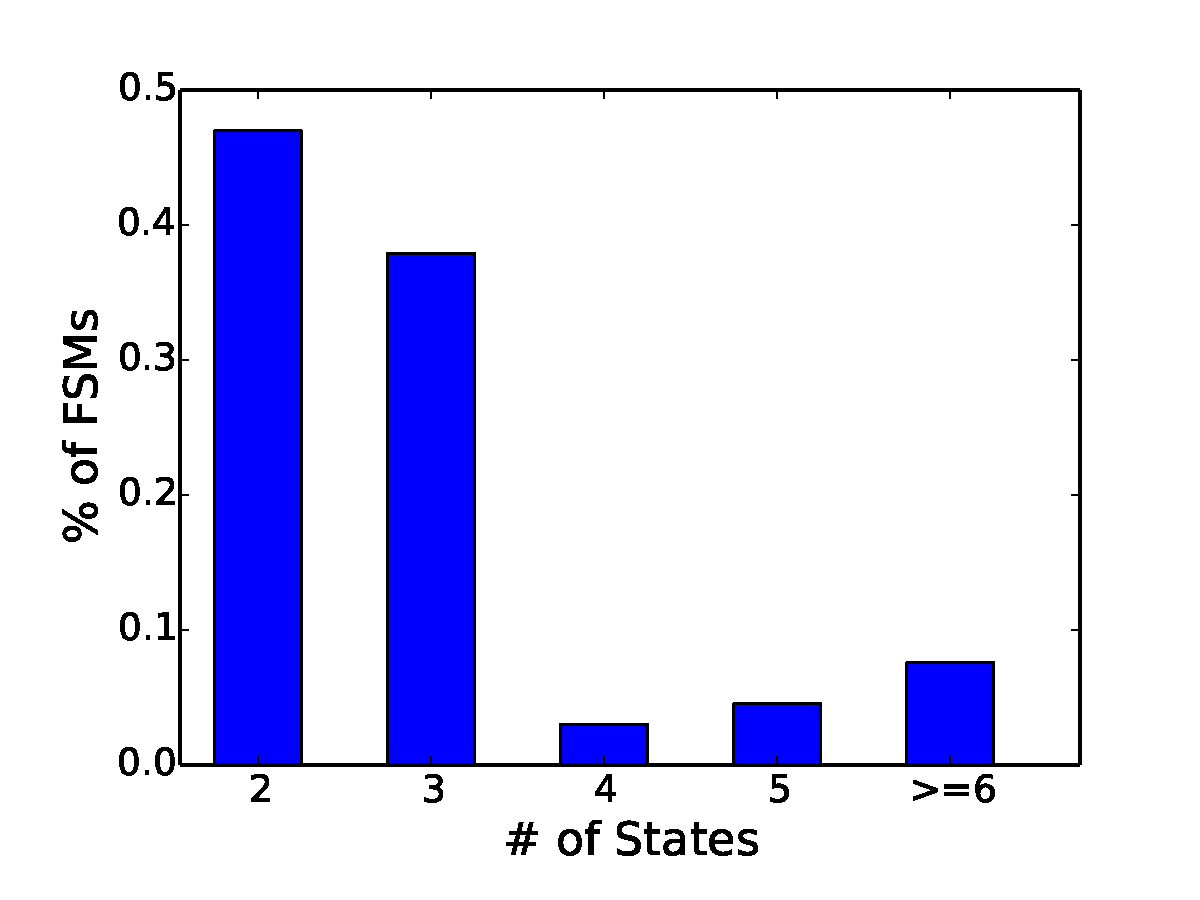
\includegraphics[width=2.5in]{figure/sv-dist.pdf}}
%\vspace{-0.05in}
\mycaption{fig:sv}{How the number of states distributes across all identified FSMs.}
{}
\end{center}
\end{minipage}
%\vspace{0.1in}
\end{figure}
}

Figure~\ref{fig:sv} shows the percentage of the identified FSMs
for different state numbers. 
More than 80\% of FSMs contain either two states or three states. 
The percentage drops significantly when the state number is larger than three. 
There are two FSMs containing 11 states. 
These two FSMs have the largest state numbers among all the identified FSMs. 
On average, one identified FSM has 3.02 possible states. 
Figure~\ref{fig:sv} also shows how the percentage of FSMs distributes 
across different state numbers 
for the 25 studied FSMs. 
The average state number for the studied FSMs is 3.84.
We use chi-square goodness of fit test to compare 
the two distribution in Figure~\ref{fig:sv}. 
The testing result shows that there is no significant 
difference between the two distributions 
under 99\% confidence level. 
Our study results in Section~\ref{sec:study} are general enough to be 
extended to other data sets. 

\noindent\textbf{Accuracy.}
As shown in Table~\ref{tab:exp}, \Tool{} is accurate. 
It only has two false positives.
The false-positive-vs-FSM rate is 1:35. 

The two false positives are caused due to the same reason. 
In each case, an integer variable is used to hold a function pointer. 
The identified FSM loop checks whether the integer variable is \texttt{0}. 
If so, the integer variable is assigned with a constant number, 
which is actually the address for the entry point of a function. 
\Tool{} identifies the integer variable as a state variable.  
In future, we plan to extend \Tool{} by examining how identified 
state variables are used beyond FSM 
loops to filter out similar false positives. 
Take the FSM in Figure~\ref{fig:cgc} as an example, 
to trigger the program to execute line 20, 
a fuzzer needs to generate an input \verb/|("[^"]*")?|/






\section{Applications}
\label{sec:app}

%\Tool{} is a tool that can automatically extract implemented FSMs in a program.
In this section, we will discuss how the extracted FSMs can facilitate
various network and security practices.


\noindent\textbf{Network Verification.}  In network operation, before a network
is deployed into production, its configuration needs to be verified to avoid
runtime errors. In such a network verification process, network operators
usually build behavior models for individual network appliances and then
reason about the end-to-end properties of the
network~\cite{mai2011debugging,khurshid2013veriflow,kazemian2012header,kazemian2013real,fayaz2016buzz,panda2017verifying}.
FSM is an expressive
behavior model to represent a wide range of network appliances, including
switches and software network functions (e.g. load balancers, firewalls, NAT). 
With individual FSMs and the network topology ready, the network
operator could verify whether the communication between end hosts satisfies
properties (e.g. reachability, isolation, loop-freedom).%~\cite{xxx}.

\Tool{} is helpful in the procedure of ``building behavior models for
individual network appliances'', which currently is manually crafted by
the network operators by reading the code or according to their
empirical understanding. \Tool{} can primarily automate the
transformation from network software to FSMs. More importantly, it
provides the confidence that the output FSM is logically equivalent
to the original software.


\noindent\textbf{Code Debloating.}
Code bloat refers to codes in an unnecessarily large size~\cite{code-bloat}.
It widely exists in production-run software~\cite{code-bloat-study}.
If untackled, bloated codes can introduce vulnerabilities~\cite{protocol-mao} and 
degrade the software performance~\cite{BloatFSE2008,XuBloatPLDI2009,XuBloatPLDI2010}.
Many techniques are proposed to address the code bloating problem.
They either remove temporary object copies~\cite{BloatFSE2008,XuBloatPLDI2009,
XuBloatPLDI2010,Reusable,Cachetor}
or eliminate functions unreached from
\texttt{main}~\cite{container-debloating-1,
container-debloating-2, dinghao-1}.
None of them change the underlying program models.
With extracted FSMs from \Tool{},
further code debloating can be performed through
eliminating unnecessary program logics.
For example, given the extracted FSM in Figure~\ref{fig:cgc},
developers may consider removing state \texttt{open\_double} and
\texttt{close\_double}.
A tool can take the FSM as input and automatically
remove code pertaining to the two states.
The tool can test or validate the changed program
by monitoring the control flow
in the FSM loop and the value of the state variable.

\noindent\textbf{Fuzz Testing.}
Fuzzing is an automated testing technique,
which executes a program
using randomly mutated inputs
with the goal to trigger unexpected program behaviors,
such as crashes and assertion errors~\cite{afl,Angora,youwei-1}.
Fuzzers are usually evaluated by measuring code coverage.
A better fuzzer can cover more lines of code
or branches under a given time constraint.
The state-of-the-art fuzzers are not good at processing
FSMs in a program.
Take the FSM in Figure~\ref{fig:cgc-fsm} as an example,
``\verb/||/'' is the only input which has two characters and
can transit the program to state \texttt{close\_set} at line 20.
If a fuzzer completely relies on random mutation, the probability to
generate ``\verb/||/'' is very low ($1/(256 * 256)$).
However, if the fuzzer is enhanced by the
FSM in Figure~\ref{fig:cgc},
it will easily figure out how to create inputs to quickly cover
all states and state transitions.







\section{Related Works}
\label{sec:related}

\noindent\textbf{Program analysis to extract models.}
A set of work also applies program analysis techniques
to extract certain models implemented in programs:
for example, NFactor~\cite{wu2016automatic}
uses symbolic execution and program slicing to extract match-action
tables in NF programs;
StateAlyzr~\cite{khalid2016paving} extracts state abstractions
from implementations of stateful protocols.
Different from existing techniques, \Tool{} extracts FSMs,
which are more concise and expressive.

\noindent\textbf{Blackbox modeling.}
Another approach to get the FSM of a program is blackbox modeling.
L* algorithm invented by~\citet{angluin1987learning}
is the theoretical foundation.
It executes a program with different inputs and
synthesizes the FSM by observing outputs.
L* algorithm is applied in various scenarios
(e.g. NF modeling~\cite{moon2019alembic},
protocol analysis~\cite{cho2011mace}).
Compared with \Tool{}, blackbox approaches suffer from two limitations.
First, they model the whole program as one single FSM in a coarse granularity,
while it is possible that there are multiple FSMs in a program.
Second, their completeness and soundness are limited,
since it is difficult to enumerate all inputs for
FSM inference.



\section{Conclusions}

Automatically extracting FSMs in a program is important
and challenging.
In this paper, we tackle this problem by building a tool, \Tool{},
which relies on static analysis to identify and synthesize implemented FSMs.
Our evaluation shows that \Tool{} successfully identifies all FSMs and
reports very few false positives.
In the future, we plan to combine \Tool{} with existing network verification
or fuzzing techniques to build end-to-end network or security applications.









%%\balance
%\begin{spacing}{0.65}

\balance
{
\bibliographystyle{abbrvnat}
\bibliography{fsm} 
}
%\end{spacing}
\end{document}
